\documentclass[12pt]{article}

\usepackage{amssymb}
\usepackage{graphicx}
\usepackage{amsmath}
\usepackage[utf8]{inputenc}

\title{Dokumentation "FINd die Werwölfe"}
\author{Alexandra Koch, Gina Seckendorf, Jonathan Kloss}

\begin{document}

\maketitle
\begin{center} 
\includegraphics{wolf} \end{center}
\tableofcontents
\setcounter{tocdepth}{3}

\newpage

\section{Projektidee}

\subsection{Spielbeschreibung}
Als Vorlage für die App dient das Spiel $"$Die Werwölfe von Düsterwald$"$ von Philippe des Phalliéres und Hervé Marly. Thematisch geht es darum, dass das kleine Dörfchen Düsterwald von Werwölfen heimgesucht wird. Die Gruppe der Bürger versucht die Wölfe, die sich als Bürger getarnt haben, zu entlarven. Dagegen versuchen die Wölfe als einzige zu überleben und Widersacher auszuschalten.

\subsubsection{Vorbereitung}
Der Spielleiter mischt alle Charakterkarten und teilt an jeden Spieler verdeckt eine davon aus. Die Spieler schauen sich ihre Karte an und erkennen nun, ob sie einen Werwolf, einen einfachen Dorfbewohner oder eine Sonderrolle verkörpern. Danach ruft der Spielleiter zur ersten Nacht aus und das eigentliche Spiel kann beginnen.

\subsubsection{Nachtphase}
In der Nachtphase schließen alle Spieler die Augen. Der Spielleiter ruft die handelnden Charaktere einzeln auf. Sie öffnen ihre Augen und führen ihre Aktion aus.

\vspace{0,3 cm}

Der \textit{Dieb} ist der erste, der im Spiel erwacht. Wird mit Dieb gespielt, werden zwei Karten mehr ausgeteilt. Der Dieb darf diese ansehen und seine Karte gegen eine der beiden übrig gebliebenen Karten austauschen. Er hat ab jetzt also eine neue Rolle. Möchte er nicht tauschen, ist er für den Rest des Spiels einfacher Dorfbewohner.

\vspace{0,3 cm}

\textit{Amor} erwacht nur einmal in der allerersten Nacht, um zwei Spieler seiner Wahl miteinander zu
verkuppeln (eventuell auch sich selbst). Danach schläft er wieder ein. Anschließend berührt der
Spielleiter die beiden Verliebten an der Schulter, sodass diese kurz erwachen können und wissen,
wer der jeweilige Partner ist. Die Verliebten haben im Laufe des Spiels die Aufgabe, den Partner
zu beschützen, denn wenn einer der beiden stirbt, macht es ihm der Partner trauernd nach; sie
dürfen nie gegeneinander stimmen.

\vspace{0,3 cm}

Werden die \textit{Werwölfe} vom Spielleiter aufgerufen, wachen sie auf und erkennen sich gegenseitig.
Je nach Spielerzahl gibt es zwei bis vier Wölfe. Die Wölfe einigen sich durch Gesten auf ein Opfer und schlafen dann wieder ein.
Der Spielleiter merkt sich das Opfer der Werwölfe.

\vspace{0,3 cm}

Das kleine \textit{Mädchen} darf nachts in der Werwolf$-$Phase heimlich blinzeln, um so die Werwölfe zu
erkennen. Die Werwölfe ihrerseits hingegen achten natürlich darauf, das Mädchen dabei zu ertappen,
es besteht also beim Blinzeln ein gewisses Risiko.

\vspace{0,3 cm}

Die \textit{Seherin} erwacht in der Nacht alleine und zeigt auf einen Spieler.
Der Spielleiter zeigt der Seherin nun die entsprechende Charakter-Karte der Person.
Die Seherin weiß dadurch mehr als die übrigen Dorfbewohner, muss aber mit ihrem Wissen
sorgfältig umgehen, um nicht von den Werwölfen enttarnt zu werden.

\vspace{0,3 cm}

Die \textit{Hexe} erwacht immer nachdem die Werwölfe ihr Opfer ausgesucht haben.
Sie hat im Verlauf des gesamten Spiels einen Gift- und einen Heiltrank.
Der Spielleiter zeigt auf die Person, die von den Werwölfen als Mordopfer gewählt wurde und die
Hexe kann diese mit ihrem Heiltrank heilen (auch sich selbst), so dass es am nächsten Morgen keinen
Toten gibt. Sie kann aber auch den Gifttrank auf einen anderen Spieler anwenden $-$ dann gibt es mehrere Tote.

\vspace{0,3 cm} 

Scheidet der \textit{Jäger} aus dem Spiel aus, feuert er in seinem letzten Atemzug noch einen Schuss ab,
mit dem er einen Spieler seiner Wahl mit in den Tod reißt, d.h. er bestimmt einen Spieler,
der mit ihm aus dem Spiel ausscheidet.

\subsubsection{Tagphase}
Am Tag wachen alle Spieler auf. Das Opfer der Werwölfe wird verkündet, es dreht seine Karte um,
gilt als tot und scheidet aus der Runde aus, d. h., er darf keinen Kommentar zum Spiel mehr abgeben.
Nun diskutieren die Dorfbewohner, wer von ihnen ein Werwolf sein könnte. Diese Diskussionsphase
ist das eigentliche Herzstück des Spiels.

\vspace{0,3 cm}
Am Ende des Tages gibt es eine sogenannte Abstimmung durch das Dorfgericht, wobei auf Kommando des
Spielleiters jeder, außer den ausgeschiedenen Personen, mit dem Finger auf eine für ihn verdächtige
Person deutet. Wer die meisten Stimmen erhält, scheidet aus. Bei Gleichstand gibt es eine Stichwahl,
bei erneutem Patt entscheidet ein zu Spielbeginn gewählter Hauptmann. Den verbleibenden Spielern
wird die Charakterrolle des ausgeschiedenen Spielers bekanntgeben. Nach dem Tag wird es wieder
Nacht und der Zyklus beginnt von vorn.

\subsubsection{Ende des Spiels}
Das Spiel endet, sobald entweder alle Werwölfe oder alle Bürger tot sind.
Das Ziel der Werwölfe ist es, alle Bürger auszulöschen, während die Dorfbewohner den Wölfen den
Garaus machen wollen. Lediglich wenn das Liebespaar aus einem Werwolf und einem Dorfbewohner besteht,
können diese beiden Spieler nur dann gewinnen, wenn außer ihnen niemand überlebt.

\subsection{Idee: Umsetzung als Android-App}
Die App versucht das Spiel so gut wie möglich digital umzusetzen. Die Spielkarten werden durch ein Android$-$Gerät ersetzt und ein Spielleiter ist nicht mehr notwendig. Alle notwendigen Daten werden in einer Datenbank gespeichert. So kann jedes Gerät jederzeit darauf zugreifen.
Der Spielablauf soll nun wie folgt aussehen: 
Jeder Spieler benötigt zum Spielen sein Smartphone mit der $"$FINd die Werwölfe$"-$App mit einen Spieler$-$Account. Ein Spieler kann nun ein neues Spiel erstellen. Dadurch wird ein QR-Code erstellt, welchen die anderen Spieler scannen können, um diesem Spiel beizutreten. Die Rollen werden den Spielern automatisch und zufällig zugewiesen. Sobald alle Spieler bereit sind, kann das Spiel beginnen. Wie im Kartenspiel haben die Spieler die Augen während der Nachtphase geschlossen. Audio$-$Ausgaben leiten die Spieler durch das Spiel und fordern die Spieler zum Öffnen$/$Schließen ihrer Augen auf. Diese werden vom $"$Spielleiter$"-$Gerät (\textit{Gerät des Spielers, der das Spiel erstellt hat}) abgespielt. In der Nacht erwachen nach und nach die Sonderrollen und führen ihre Aktionen auf dem Gerät aus. Am Tag sehen dann alle Spieler auf ihren Geräten welche Opfer es in der Nacht gegeben hat. Danach werden den Spielern Buttons von allen Spielern angezeigt. Aus diesen können sie dann das Opfer des Tages wählen.
Die Geräte stehen in ständiger Verbindung zur Datenbank, um zu wissen in welcher Phase sich das Spiel befindet und wann das Ende des Spiels erreicht ist. 



\section{Umsetzung}

	\subsection{Projektplanung}
	
Zur Implementierung der App wurde Android-Studio verwendet. [Datenbank auf Server] $\dots$	
	
		
		\subsubsection{Meilensteine}
		
\begin{enumerate}

\item \textbf{Aufgabenplanung} \\
$\rightarrow$  

\item \textbf{Modellierung der App} \\
$\rightarrow$

\item \textbf{Recherche} \\
$\rightarrow$ Informieren über die Techniken und Werkzeuge zur Umsetzung der App

\item \textbf{Implementierung} \\
$\rightarrow$ Umsetzung aller Funktionen in Android$-$Studio

\item \textbf{Datenbank} \\
$\rightarrow$ Implementierung der php-Files zur Kommunikation zwischen Datenbank und Android$-$Geräten

\item \textbf{Design} \\
$\rightarrow$ optische und akustische Gestaltung der App

\item \textbf{Dokumentation} \\
$\rightarrow$ Erklärung für Entwickler und Benutzer wie die App funktioniert

\item \textbf{Testen} 

\item \textbf{Abschlusspräsentation} 


\end{enumerate}
		
		
		\subsubsection{Projektplan}



		\subsubsection{Burn-Down-Chart}




	\subsection{Projektdurchführung}
		
		\subsubsection{Klassendiagramm}
		
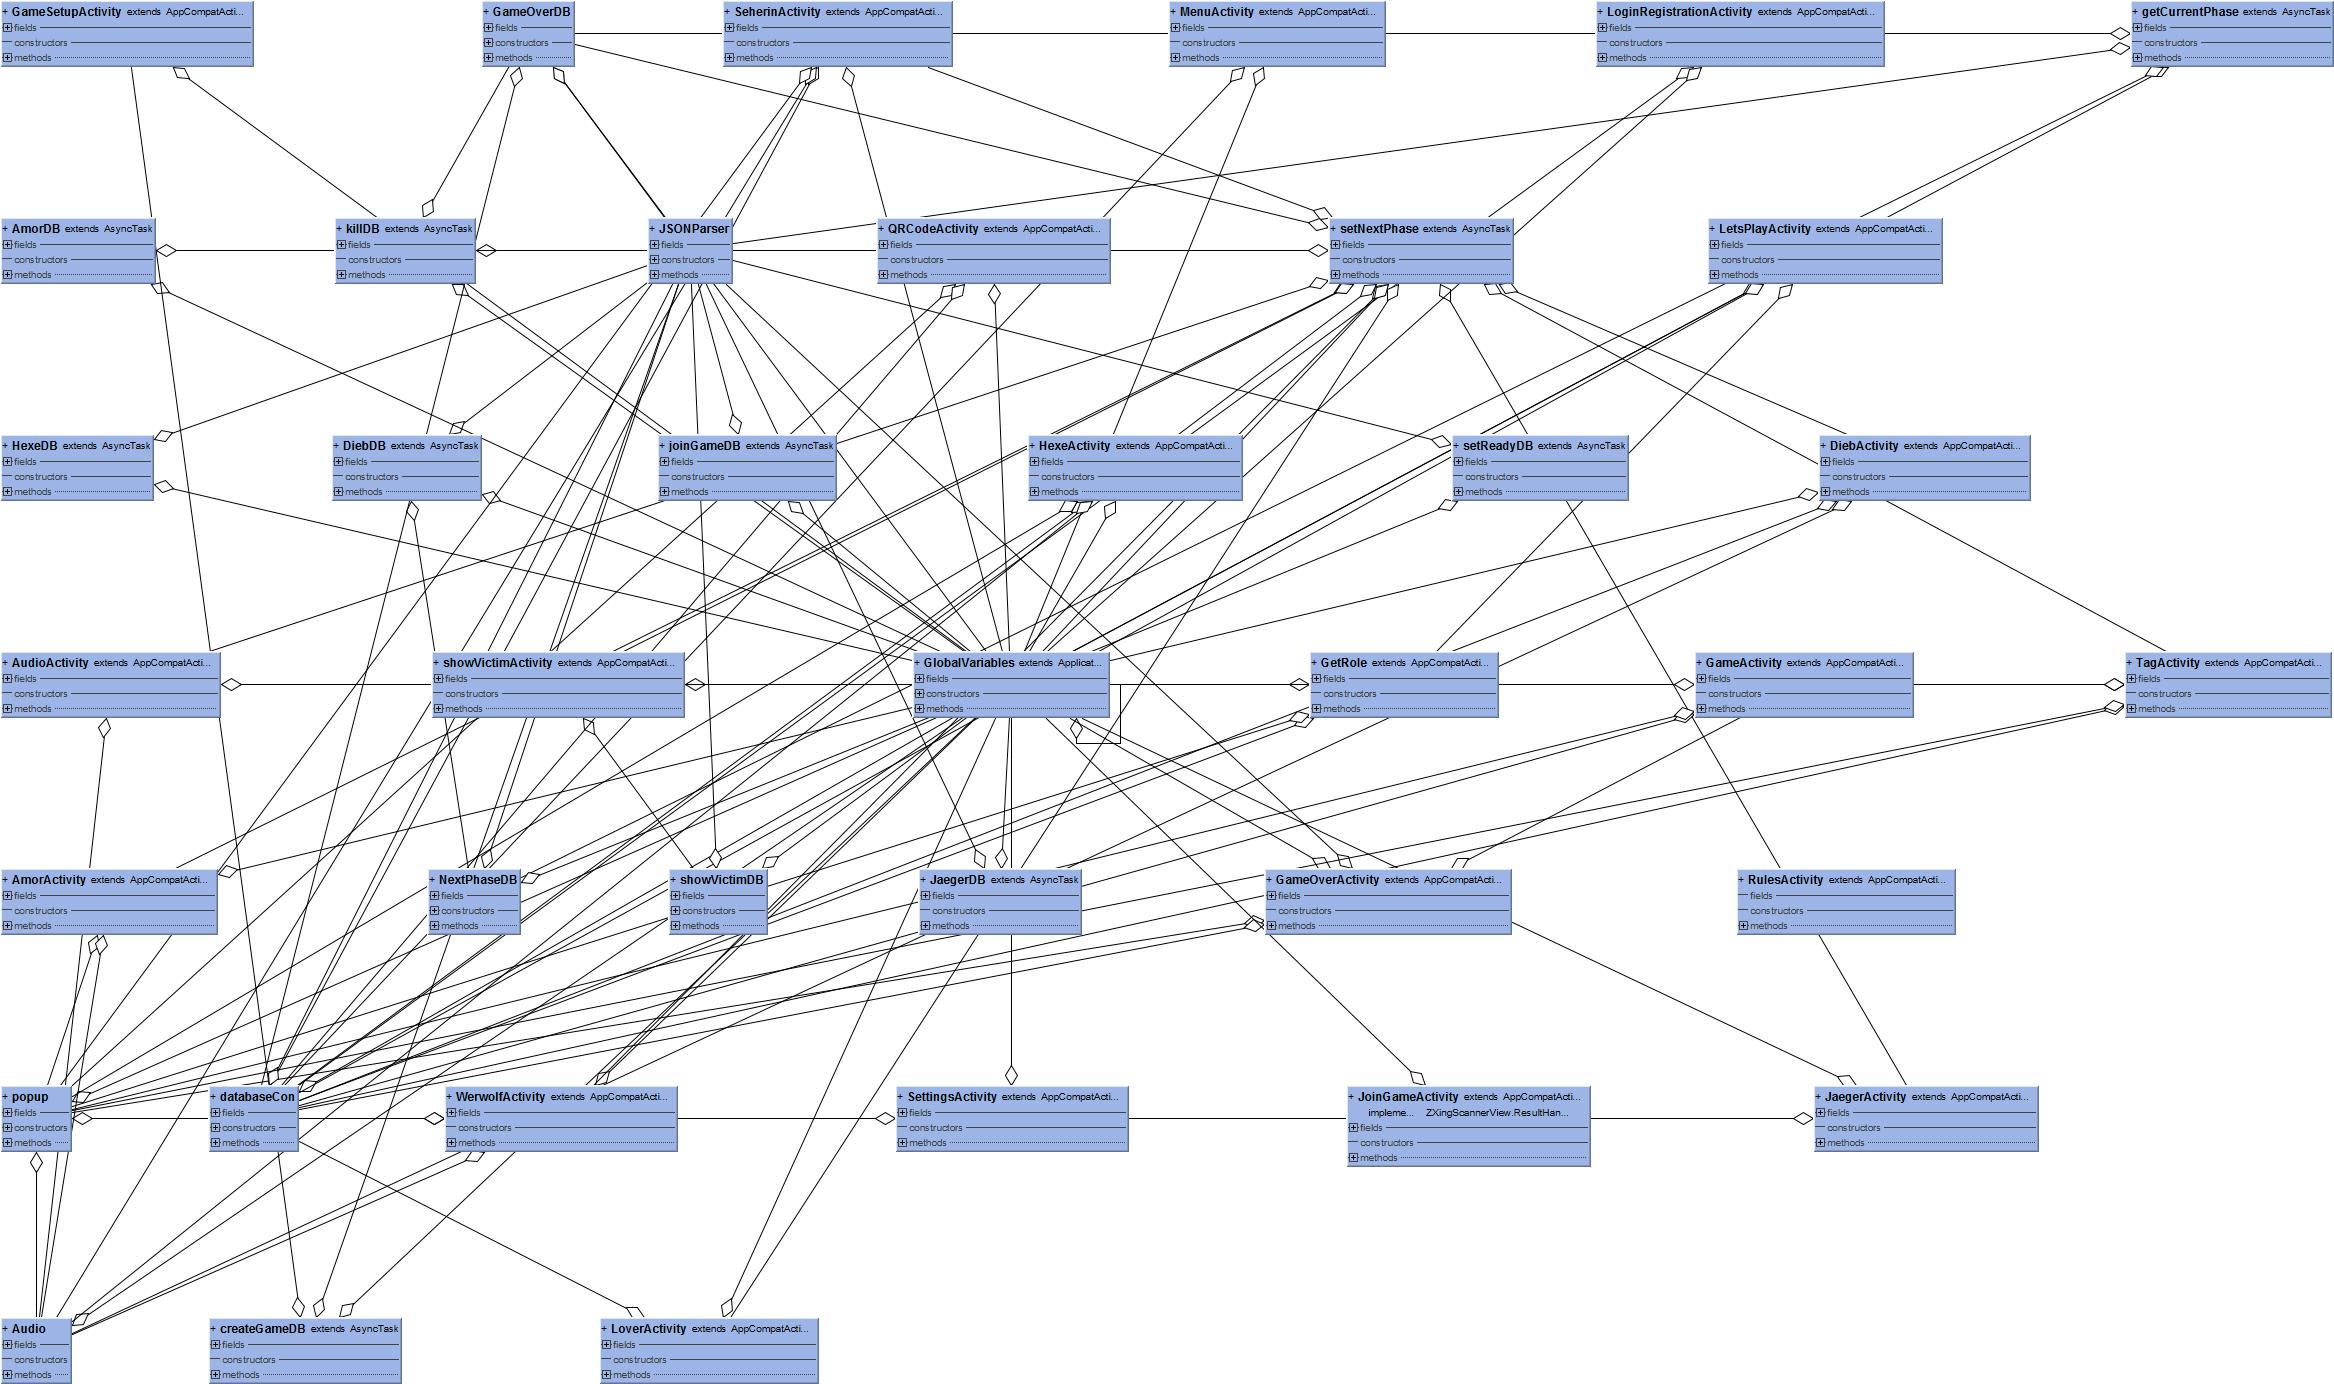
\includegraphics[width = 15 cm, height = 8 cm]{WUML}
		
		
		\subsubsection{Beschreibung der Klassen}
		
\textbf{AmorActivity.}
Zu Beginn der Activity wird über das Spielleiter-Gerät ein Audio abgespielt, welches Amor auffordert die Augen zu öffnen. Diesem wird nun auf dem Display die Spieler anzeigt, welche mit Hilfe der Methode createObjects der Klasse \textit{GameActivity} erstellt werden. Allen anderen Spielern wird ein schwarzer Bildschirm angezeigt (activity$\_$wait layout). Amor kann nun zwei Spieler (auch sich selbst) wählen. Seine Wahl bestätigt er mit dem $"$Bestätigen$" -$ Button. Damit wird die Klasse \textit{AmorDB} aufgerufen und die gewählten Spieler werden in der Datenbank mit ihrem jeweiligen Liebespartner abgespeichert (setLovers()).
Über ein PopUp der Klasse \textit{popup.java} wird Amor noch einmal das Liebespaar angezeigt. Mit dem Klick auf OK wird die nächste Phase aufgerufen (new setNextPhase().execute($"$audio$");)$.

\vspace{0,3 cm}
      
\textbf{AudioActivity.}
Diese Activity wird nach jeder Phase aufgerufen (new setNextPhase().execute($"$audio$");)$, um dem Spieler zu sagen, dass dieser wieder einschlafen/die Augen schließen soll. Sie zeigt einen schwarzen Bildschirm und lässt vom Spielleiter-Gerät das entsprechende $"$Einschlaf-Audio$"$ abspielen. Dazu ruft sie die Klasse \textit{Audio} auf.

\vspace{0,3 cm}

\textbf{DiebActivity.}
Aus dieser Activity werden zuerst die beiden übrig gebliebenen Rollen aus der Datenbank geladen. Diese werden zusammen mit dem entsprechenden Bild und der Beschreibung auf zwei Buttons dargestellt.
Der Dieb bekommt zwei Rollen angezeigt. Diese werden mit Hilfe der Methode \textit{DiebGetRole} der Klasse \textit{databaseCon} aus der Datenbank abgefragt. Diese Rollen werden mit Hilfe der Rollenkarten auf dem Display des Diebs dargestellt. Wählt er eine aus, so wird ihm die Rollenbeschreibung in einem PopUpChoice$-$Fenster angezeigt, welches mit Hilfe der Klasse \textit{popup} erstellt wurde und er kann wählen, ob er sich für oder gegen diese Rolle entscheiden will. 
Sind beide wählbaren Rollen Sonderrollen, so bekommt der Dieb auch die Möglichkeit durch einen Extrabutton, dass er ein einfacher Dorfbewohner bleiben kann. Ist eine mögliche Wahl ein Werwolf, so hat der Dieb keine andere Wahl, als ein Werwolf zu werden. Es erscheint somit, bevor der Dieb eine Wahl treffen kann, ein PopUp$-$Fenster der Klasse \textit{popup}, welches ihm mitteilt, dass er von nun an als Werwolf weiter spielen wird. Hat der Dieb seine Wahl getroffen oder das $"$Werwolf$-$Info$-$PopUp$"$ geschlossen, so wird die \textit{DiebDB.java} ausgeführt. 
Nachdem sich der Spieler seine Entscheidung getroffen hat, wird die Auswahl in den globalen Variablen sowie in der Datenbank gespeichert. Anschließend wird die nächste Phase wird aufgerufen.

\vspace{0,3 cm}
      
\textbf{HexeActivity.}
Zuerst bekommt die Hexe angezeigt, wer das Opfer der Werwölfe ist.
Sollte sie noch einen Heiltrank zur Verfügung haben, hat sie die Wahl, ob sie das Opfer retten möchte. 
Dies wird mithilfe der \textit{databaseCon} in der Datenbank gespeichert.
Sollte sie noch einen Gifttrank zur Verfügung haben, wird gefragt, ob sie diesen verwenden möchte.
Wenn sie sich dafür entscheidet, darf sie einen Spieler auswählen, der sterben soll.
Andernfalls wird die nächste Phase aufgerufen.
Auch diese Wahl wird mithilfe der \textit{databaseCon} in der Datenbank gespeichert.
      
\vspace{0,3 cm}      
      
\textbf{JaegerActivity.}
Diese Activity wird aufgerufen, sobald der Jaeger gestorben ist. Über ein PopUp wird er aufgefordert einen Spieler auszuwählen, der mit ihm sterben soll. zur Auswahl werden ihm alle Spieler angezeigt. Sobald er ein Wahl getroffen hat und diese mit OK bestätigt, wird die \textit{JaegerDB} aufgerufen.
Allen anderen Spielern wird derweil ein Infotext angezeigt und mit $"$timerHandler.postDelayed(timerRunnable, 2000)$;"$ warten sie auf die nächste Phase.
    
\vspace{0,3 cm}    
      
\textbf{LoverActivity.}
Alle Spieler werden durch ein Audio aufgefordert die Augen zu öffnen, um auf ihrem Display zu sehen, ob sie in eine andere Person verliebt sind. Das Audio fordert sie auch auf wieder einzuschlafen. Im Anschluss wird die nächste Phase aufgerufen.

\vspace{0,3 cm}

\textbf{SeherinActivity.}
Die Seherin wird durch ein PopUp$-$Info$-$Fenster der Klasse \textit{popup} aufgefordert, einen Spieler zu wählen, dessen Gesinnung er erfahren möchte. Die Wahl erfolgt über durch die Methode \textit{createObjects} der Klasse \textit{GameActivity} erstellte Spieler$-$Icons. Wählt der Spieler einen anderen Spieler aus, so erscheint ein PopUp$-$Info$-$Fenster der Klasse \textit{popup}, welches dem Spieler mitteilt, ob der von ihm gewählte Spieler gut (Dorfbewohner oder Sonderrolle) oder böse (Werwolf) ist. Diese Informationen werden mit Hilfe der Methode \textit{getIdentity}, welche die Methode Seherin der Klasse \textit{databaseCon} aufruft, erhalten. Bestätigt der Spieler die Informationen mit Betätigung des $"$OK$"-$Buttons des  PopUp$-$Info$-$Fensters, so wird \textit{setNextPhase} aufgerufen. Anschließend wird die nächste Phase aufgerufen.

\vspace{0,3 cm}      
   
\textbf{showVictimActivity.}
In dieser Activity werden die Opfer angezeigt.
Mögliche Gründe dafür sind die Abstimmung der Dorfbewohner am Tag, die Wahl der Werwölfe in der
Nacht, der Gifttrank der Hexe, der Schuss des Jägers oder ein gestorbener Liebender.
Nach einer gewissen Zeit wird automatisch die nächste Phase aufgerufen.

\vspace{0,3 cm}      
      
\textbf{TagActivity.}
Am Tag erwachen alle Spieler, die noch am Leben sind. 
Sie können ihre Stimme für denjenigen abgeben, den sie töten möchten. Ihre Auswahl wird in der Datenbank
gespeichert. Anschließend warten das Gerät auf ein Ergebnis der Abstimmung.
Das Gerät des Spielleiters kontrolliert dabei, ob alle Spieler ihre Stimme abgegeben haben.
Sollte das der Fall sein, wird der Spieler mit den meisten Stimmen als \textit{victimDor} in der Datenbank
gespeichert      

\vspace{0,3 cm}

\textbf{WerwolfActivity.}
In dieser Phase erwachen die Werwölfe und wählen per Klick auf einen Button ihr Opfer.
Die Auswahl wird in der Datenbank vermerkt. Das Gerät des Spielleiters kontrolliert regelmäßig,
ob alle Wölfe ihre Stimme abgegeben haben. Sollte dies der Fall sein, wird der Spieler mit den meisten
Stimmen als \textit{opferWer} in der Datenbank gespeichert.
Anschließend wird die nächste Phase aufgerufen.

\vspace{0,3 cm}

\textbf{GameActivity.}
Diese Activity ist die Grundlage für alle kommenden Spielphasen. Die \textit{createObjects}$-$Methode ist für die Erstellung aller benötigten Darstellungselemente zuständig. Das Display wird zunächst in vier Layouts geteilt, die nach und nach (je nach Anzahl der Spieler) mit Player$-$Buttons befüllt werden. Durch einen langen Klick, kann das dazugehörige Spieler$-$Bild angezeigt werden. Spieler$-$Buttons von toten Spielern sind nicht anwählbar.
Die Methode \textit{playerSelected} wird von einem Button bei einem aufgerufen und ist dafür zuständig die aktuelle Auswahl visuell darzustellen.
Nach dem erstellen der benötigten Elemente wird \textit{getCurrentPhase} aufgerufen. Diese Methode überprüft, ob eine neue Phase aktiv geworden ist und ruft die dementsprechende Activity auf. Das Spielleitergerät kündigt die jeweils folgende Phase an.
Zu Beginn einer $"$Rollen$"-$Activity wird kontrolliert, ob der entsprechende Spieler erwachen soll oder nicht. Die Displays der Spieler mit den entsprechenden Rollen gehen an und Aktionen können ausgeführt werden.
Sollte eine einzeln aufgerufene Rolle bereits gestorben sein, passiert nichts und nach einer
gewissen Zeit wird automatisch in die nächste Phase geschaltet.

\vspace{0,3 cm}
            
\textbf{GameOverActivity.}
Sobald eine Bedingung für das Ende des Spiels erfüllt ist (siehe Punkt 1 $"$Ende des Spiels$"$) wird diese Activity aufgerufen.
Über ein PopUp wird jedem Spieler angezeigt, wer gewonnen hat (Text abhängig von Rolle und Gewinner$-$Team).
Mit dem Klick auf den ENDE$-$Button gelangt man zurück ins Menü. Dabei werden alle Spiel$-$spezifischen Daten aus der Datenbank gelöscht.

\vspace{0,3 cm}
      
\textbf{GameSetupActivity.}
Diese Activity lässt den Spieler die Einstellungen für das zu erstellende Spiel treffen.
Es gibt einen \textit{NumberPicker} für die Auswahl der Anzahl der Spieler.
Außerdem existiert ein \textit{Spinner}, der automatisch die benötigte Anzahl an Werwölfen mithilfe der Funktion \textit{setRecommendedNumberOfWer(int players)} berechnet. Es steht dem Spieler frei die Anzahl im Nachhinein zu verändern.
Im Folgenden können die Extrarollen an$-$ bzw. abgewählt werden.
Bei jeder Änderung erfolgt ein Aufruf der Funktion \textit{calculateGame}. Diese berechnet anhand der Anzahl der Werwölfe und der Anzahl der Extrarollen die benötigte Anzahl an Dorfbewohnern für das Spiel und setzt diese automatisch.
Alle teilnehmenden Rollen werden in das \textit{cards}$-$Array geschrieben, welches anschließend gemischt wird
und das \textit{cardsShuffled}$-$Array entsteht.
Die für das Spiel benötigten Phasen werden gesammelt und die \textit{createGameDB()} wird ausgeführt.
Die Phasen sowie die Rollen werden in die Datenbank geschrieben.
Nach erfolgreicher Erstellung des Spiels in der Datenbank wird die \textit{QRCodeActivity} aufgerufen. Das Gerät des Spieler, der das Spiel erstellt hat, wird zum $"$Spielleiter$"-$Gerät.
\vspace{0,3 cm}  

\textbf{GetRole.}
Mit dem Aufruf dieser Activity wird die der Spielerrolle entsprechenden Karte geladen und kann durch eine Betätigung des Kartensymbols angezeigt werden. Bei einer weiteren Betätigung dieses wird dem Spieler die seiner Rolle entsprechenden Rollenbeschreibung angezeigt. Berührt er die Karte erneut, so wird wieder nur die Kartenrückseite angezeigt (die Rolle bleibt verborgen). Ist der Spieler bereit, so betätigt er des $"$Bereit$"-$Button. Sobald alle Spieler bereit sind, wird die \textit{LetsPlayActivity} aufgerufen.

\vspace{0,3 cm}      
      
\textbf{JoinGameActivity.}
In dieser Activity kann der Spieler einen, auf einem anderen Handy erzeugten, QR-Code scannen.
Dieser codiert die entsprechende \textit{GameId} für das Spiel, dem beigetreten werden soll.
Mithilfe dieser Information wird in der Datenbank der Spieler dem Spiel hinzugefügt.
Anschließend wird \textit{GetRole} aufgerufen.

\vspace{0,3 cm}
      
\textbf{LetsPlayActivity.}
Diese Activity dient als Überleitung zum eigentlichen Spiel. Hierbei wird ein Audio von dem Spielleitergerät abgespielt, welches eine kurze Einleitung gibt und die Spieler auffordert die Augen zu schließen. Außerdem werden durch die Aufrufe der Methoden \textit{getPlayerIDs}, \textit{getPlayerNames} und \textit{getImagesAsString} der Klasse \textit{databaseCon} die im Spiel befindlichen \textit{PlayerIDs} und zugehörigen Namen sowie Bilder aus der Datenbank geladen und anschließend global gespeichert. Somit stehen diese zu späteren Zeitpunkten zur Verfügung und müssen nicht bei Gebrauch von der Datenbank abgefragt werden. 
Anschließend wird die \textit{GameActivity} aufgerufen.

\vspace{0,3 cm}      
     
\textbf{LoginRegistrationActivity.}
Jeder neue Spieler muss sich einen Account erstellen. Dazu wird ein neuer Eintrag in der Datenbank mit \textit{playerID}, \textit{name}, \textit{username}, \textit{password} und \textit{image} angelegt. Die Registrierung erfolgt mithilfe der Klasse \textit{databaseCon} über die Methode \textit{registration}. Bereits registrierte User können sich einfach einloggen. Der Benutzername und das Passwort werden mithilfe der Methode \textit{login} verifiziert.
Anschließend wird die \textit{MenuActivity} gestartet.

\vspace{0,3 cm} 
     
\textbf{MenuActivity.}
In dieser Activity kann sich der Spieler entscheiden, ob er ein neues Spiel starten möchte, welches
die \textit{GameSetupActivity} startet.
Andernfalls kann er einem Spiel beitreten, mittels der \textit{JoinGameActivity}, oder er öffnet die Einstellungen, wobei die \textit{SettingsActivity} geöffnet wird.
Ebenfalls möglich ist das Betrachten der Regeln \textit{Rules}.

\vspace{0,3 cm}
      
\textbf{QRCodeActivity.}
Diese Activity erzeugt aus der \textit{gameID} des erstellten Spiels einen QR-Code der von anderen Spielern
gescannt werden muss, um dem Spiel beizutreten. Erst, wenn alle Spieler dem Spiel beigetreten sind,  wird die \textit{LetsPlayActivity} auf dem Spielleitergerät aufgerufen. 
Wird die $"$Zurücktaste$"$ in dieser Activity betätigt, erscheint ein PopUp$-$Fenster (Aufruf \textit{popup}) bei 
welchem bestätigt werden muss, dass ins Menü zurückgekehrt werden soll. Wird diese Bestätigung vorgenommen, 
so wird die Methode \textit{resetOneGame} der Klasse \textit{databaseCon} aufgerufen. Im Zuge dessen wird das bereits erstellte
Spiel wieder aus der Datenbank gelöscht (aus den Tabellen $"$player$\_$game$"$, $"\_$GAME$"$ und $"\_$PHASES$"$) und die \textit{MenuActivity} wird aufgerufen.

\vspace{0,3 cm}
      
\textbf{RulesActivity.}
Diese Activity zeigt die Spielregeln und Rollenbeschreibungen an.

\vspace{0,3 cm}
      
\textbf{SettingsActivity.}
In der \textit{SettingsActivity} hat der Spieler die Möglichkeit sein Bild zu ändern. Die Änderung erfolgt mittels der Funktion \textit{setImage} der Klasse \textit{databaseCon}. Außerdem kann er seinen Account löschen.
  		
		
		\subparagraph{Classes}
		
\textbf{Audio.}
Diese Klasse kümmert sich um das Abspielen des richtigen Audios zur richtigen Zeit.

\vspace{0,3 cm}

\textbf{databaseCon.}
Diese Klasse enthält verschiedene Funktionen, die für die Kommunikation bzw. den Datenaustausch mit der Datenbank zuständig sind.

\vspace{0,3 cm}

\textbf{GlobalVariables.}
Die Klasse \textit{GlobalVariables} enthält diverse globale Variablen, sowie deren \textit{Getter} und \textit{Setter}, um eine Parameterübergabe zwischen Activitys und java$-$Klassen zu vereinfachen.

\vspace{0,2 cm}

\underline{Global variables$:$ Game}

\begin{description}

\item[ownPlayerID]\hfill \\ $\rightarrow$ speichert eigene PlayerID (für Login, Rollenabfrage, Spiel)
\item[ownRole]\hfill \\ $\rightarrow$ speichert eigene Rolle
\item[gameID]\hfill \\ $\rightarrow$ speichert aktuelle GameID
\item[numPlayers]\hfill \\ $\rightarrow$ speichert Spieleranzahl des aktuellen Spiels
\item[numPlayersAlive]\hfill \\ $\rightarrow$ speichert aktuelle Anzahl an "lebenden" Spielern des aktuellen Spiels
\item[PlayerIDs]\hfill \\ $\rightarrow$ Array aller PlayerIDs des Spiels
\item[PlayerNames]\hfill \\ $\rightarrow$ Array aller Spielernamen des Spiels
\item[cards]\hfill \\ $\rightarrow$ Array der gemischten Rollenkarten des aktuellen Spiels $\dashrightarrow$ wird nur vom Spielleiter gebraucht $\dashrightarrow$ nötig zur Spielerstellung (Einfügen des Spiels in die Datenbank)
\item[currentlySelectedPlayer]\hfill \\ $\rightarrow$ Button des aktuell ausgewählten Spielers
\item[Phases]\hfill \\ $\rightarrow$ Array, das alle Spiel$-$relevanten Phasen enthält $\dashrightarrow$ wird nur vom Spielleiter gebraucht $\dashrightarrow$ nötig zur Spielerstellung
\item[currentPhase]\hfill \\ $\rightarrow$ String, der aktuelle Phase wiedergibt $\dashrightarrow$ überwiegend zur Aktionsentscheidung in der popup-Klasse nötig
\item[nextPhase]\hfill \\ $\rightarrow$ String, der nächste Phase wiedergibt $\dashrightarrow$ nötig für Audios
\item[currentContext]\hfill \\ $\rightarrow$ speichert aktuelle Activity $\dashrightarrow$ ermöglicht den Aufruf einer Activity aus einer java-Klasse heraus
\item[sharedPrefContext]\hfill \\ $\rightarrow$ speichert Activity, in der sharedPreferences angewandt wird (nötig für Logout)
\item[winner]\hfill \\ $\rightarrow$ String, der den Gewinner enthält
\item[spielleiter]\hfill \\ $\rightarrow$ Boolean, welcher angibt, ob das Gerät Spielleitergerät ist, oder nicht $\dashrightarrow$ nötig zum Abspielen der Audios $\/$ Aufruf der killDB
\item[images]\hfill \\ $\rightarrow$ String$-$Array, welches die Base64$-$Strings der Bilder der Spieler des aktuellen Spiels speichert.

\end{description}
 
\vspace{0,3 cm}
 
\underline{Global variables: Dieb}

\begin{description}

\item[DiebChoosen]\hfill \\ $\rightarrow$ Boolean, welcher angibt, ob der Dieb als Sonderrolle ausgewählt wurde $\dashrightarrow$ denn wenn ja, müssen zwei weitere Karten ins \textit{cards}$-$Array aufgenommen werden $+$ wenn der Dieb ausgewählt wurde und es nur einen Werwolf gibt, darf dieser beim Mischen nicht eine der beiden letzten Karten werden (\textit{GameSetupActivity} $\dashrightarrow$ \textit{calculateGame} $+$ in der \textit{QRCodeActivity} wird ermittelt, wie viele Spieler dem Spiel bereits beigetreten sind (mit der Hilfe der Methode \textit{getPlayerInGame} der Klasse \textit{databaseCon}) somit muss bekannt sein, dass die letzten beiden Einträge frei bleiben werden.

\end{description}

\vspace{0,3 cm}    	

\underline{Global variables: Amor}

\begin{description}

\item[lover1]\hfill \\ $\rightarrow$ speichert den Button des Spielers, welchen Amor als lover1 ausgewählt hat
\item[lover2]\hfill \\ $\rightarrow$ speichert den Button des Spielers, welchen Amor als lover2 ausgewählt hat 
\item[OK]\hfill \\ $\rightarrow$ Button, welcher von Amor betätigt wird, wenn er seine Wahl getroffen hat -> global, da der Button erst auswählbar wird, wenn Amor genau zwei Spieler ausgewählt hat. Die auf die Button angewendeten Methoden finden allerdings in der GameActivity statt.

\end{description}
    	
\vspace{0,3 cm}

\underline{Global variables: Seherin}

\begin{description}

\item[PopUpSeherinIdentity]\hfill \\ $\rightarrow$ AlertDialog, welcher das PopUp$-$Info$-$Fenster darstellt, welches die Gesinnung eines Spielers zeigt. Da die Fenster nur in der \textit{OnCreate}$-$Methode einer Activity erstellt werden können, es in diesem Fall jedoch in der \textit{getIdentity}$-$Methode der \textit{SeherinActivity} erst den entsprechenden Text erhält, muss es global definiert werden.

\end{description}

\vspace{0,3 cm}    	

\underline{Global variables: Jäger}

\begin{description}

\item[JaegerDies]\hfill \\ $\rightarrow$ Boolean, welcher zu Beginn eines jeden Spiels auf $"$false$"$ gesetzt wird. Er zeigt an, ob der Jäger ein Opfer der Nacht $\/$ des Tages war $\dashrightarrow$ ist dies der Fall, so wird in der \textit{ showVictimActivity} noch nicht die \textit{killDB} nach Ablaufen der für die Anzeige vorgesehenen Zeit aufgerufen, sondern erst die \textit{JaegerActivity} aufgerufen. Des weiteren wird die Variable erneut in der \textit{showVictimActivity} gebraucht, um die Opfer der Nacht $\/$ des Tages und das$\/$die Opfer des Jägers entsprechend anzeigen zu können (es muss bekannt sein, welche Textfelder angezeigt werden sollen $-$ so gibt es eines speziell für das$\/$die Jägeropfer)
\item[victimJaeger]\hfill \\ $\rightarrow$ Boolean, der das Opfer des Jägers beinhaltet. Wird genutzt, damit die entsprechende Aktion nur ausgeführt wird, wenn der Jäger ein Opfer gewählt hat.

\end{description}
  
\vspace{0,3 cm}

\textbf{JSONParser.}

\vspace{0,3 cm}

\textbf{popup.}



		\subparagraph{Database}
		
\textbf{AmorDB.}
Diese Klasse wird als AsyncTask ausgeführt. Dabei wird eine Datenbankaktualisierung mit Hilfe des PHP$-$Files \textit{setLovers}, der Methode $"$POST$"$ und den \textit{params} lover1(\textit{params}[0]), lover2(\textit{params}[1]) durchgeführt. Im Zuge dessen werden in der $"$player$\_$game$"-$Datenbanktabelle bei den Spielern, deren playerIDs lover1 bzw. lover2 entsprechen, in der Spalte $"$lover$"$ die PlayerID des jeweils andere eingetragen.

\vspace{0,3 cm}

\textbf{createGameDB.}
Mithilfe des $"$create$\_$new$\_$game.php$"$ erstellt diese Klasse ein neues Spiel in der Datenbank. Dabei fügt sie ein neues Spiel in die $\_$GAME$-$Tabelle ein und erstellt dazu Einträge in der player$\_$game$-$Tabelle [2.2.3 Fig. 2]. Des weiteren werden die Phasen des Spiels angelegt.

\vspace{0,3 cm}

\textbf{DiebDB.}
Diese Klasse wird als AsyncTask ausgeführt. Dabei wird ein http-request mit den Parametern gameID, playerID, der neuen Rolle 
(newRole $\dashrightarrow$ aus params[0]), der Rolle, die nicht gewählt wurde (notChoosen $\dashrightarrow$ aus params[1]]) und, wenn der Dieb ein Dorfbewohner bleiben möchte, die zweite Rolle, die nicht gewählt wurde (nothingChoosen $\dashrightarrow$ aus params[2]), der Methode $"$POST$"$ und unter der Nutzung des PHP$-$Files $"$changeRole.php$"$ an die Datenbank geschickt. Im Zuge dessen wird die Rolle des Diebs entsprechend seiner Wahl geädert, die überflüssigen Rollen werden aus der $"$player$\_$game$"-$Tabelle gelöscht und, wenn nötig, wird die $"\_$PHASES$"-$Datenbanktabelle geändert. Dies geschieht, wenn der Dieb sich gegen eine Sonderrolle entscheidet. Sollte dies der Fall sein, so wird die entsprechende Phase gelöscht. Nach Abschluss der Datenbankkommunikation wird die Klasse \textit{setNextPhase} aufgerufen.

\vspace{0,3 cm}

\textbf{GameOverDB.}
Diese Klasse überprüft regelmäßig, ob eine Bedingung für das Ende des Spiels erfüllt ist. Wenn ja, ändert sie dementsprechend die globale Variable \textit{winner}.

\vspace{0,3 cm}

\textbf{getCurrentPhase.}
Diese Klasse wird als AsyncTask ausgeführt. Jedes Gerät, das gerade nicht $"$aktiv$"$ ist, d.h. die Geräte der Spieler die ihre Augen geschlossen haben, erfragen periodisch mithilfe dieser Klasse die aktuelle Phase. Die aktuelle Phase wird einmal global und einmal in der Datenbank gespeichert. Unterscheiden sich diese Phasen, weiß das Gerät, dass sich die Phase geändert hat und schaltet zur nächsten Activity $\/$ Phase weiter.

\vspace{0,3 cm}

\textbf{HexeDB}
Wenn die Hexe sich dazu entschließt einen ihrer Tränke zu verwenden, wird dies durch diese Klasse in der Datenbank gespeichert \textit{updateHexe.php}.

\vspace{0,3 cm}
	
\textbf{JaegerDB.}
Diese Klasse speichert das Opfer des Jägers in der Datenbank. (\textit{setVictims.php})

\vspace{0,3 cm}

\textbf{joinGameDB.}
Sobald ein Spieler den QR-Code gescannt hat, wird er mithilfe dieser Klasse bei der passenden gameID in die player$\_$game$-$Tabelle eingefügt (\textit{insert}$\_$\textit{player.php}).

\vspace{0,3 cm}

\textbf{killDB.}
In dieser Klasse wird der \textit{alive}$-$Status der aktuellen Opfer auf 0 gesetzt und die \textit{victim}$-$Einträge in der $\_$GAME$-$Tabelle werden auf NULL (bzw. 0) zurückgesetzt. (\textit{changeAlive.php}).

\vspace{0,3 cm}
	
\textbf{NextPhaseDB.}
Diese Klasse holt sich aus der Datenbank zu einer bestimmten Phase den \textit{nextPhase}$-$Eintrag und ändert dementsprechend die globale Variable \textit{nextPhase}.

\textbf{setNextPhase.}
Am Ende jeder Phase wird vom gerade $"$aktiven$"$ Gerät die Klasse \textit{setNextPhase} aufgerufen. Diese ändert die aktuelle Phase in der Datenbank.

\textbf{setReadyDB.}
Diese Klasse ändert den \textit{ready}$-$Eintrag eines Spielers in der Datenbank (in der player$\_$game$-$Tabelle), sobald dieser in der \textit{GetRole} auf den \textit{bereit}$-$Button gedrückt hat.
	
\textbf{showVictimDB.}


		\subparagraph{php-Files}


		
\newpage	
\subsubsection{Datenbankschema}
			
Beschreibung der Tabellen in Fig.1:
\\		
		
\textbf{$player\_game.$}
Diese Tabelle ordnet einem Spieler ein Spiel zu und speichert, welche Rolle dieser verkörpert (\textit{role}). Der \textit{ready}$-$Wert ist für den Beginn des Spiels gedacht. Sobald alle Spieler dem Spiel beigetreten und bereit sind (\textit{ready == 1}) beginnt das Spiel. Bei den Abstimmungen wird in der \textit{numOfVotes} gespeichert, wie oft für einen Spieler abgestimmt wurde.
\\

\textbf{$\_GAME.$}
In dieser Tabelle werden Spiel-spezifische Informationen gespeichert. Sie enthält den Tränke-Vorrat der Hexe (\textit{poison, heal}) und die aktuell zum Tode verurteilten (\textit{victimDor, victimWer, $\dots$}).
\\

\textbf{$\_PHASES.$}
Hier werden zu jedem Spiel die notwendigen Spielphasen gespeichert. Abhängig von der Auswahl der Rollen werden diese zu Beginn des Spiels festgelegt. Die Tabelle zeigt die jeweiligen Phasen (\textit{phases}) mit ihren darauf folgenden Phasen (\textit{nextPhase}). Der Wert \textit{currentPhase} gibt an, in welcher Phase sich ein Spiel befindet.
\\

\textbf{$\_PLAYER.$}
Diese Tabelle enthält alle Spieler-Accounts. Der \textit{login}-Wert gibt an, ob ein Spieler auf einem Gerät angemeldet ist. So wird sicher gestellt, dass jeder Spieler nur auf einem Gerät angemeldet sein kann.  

\begin{figure}[] 
  \centering
     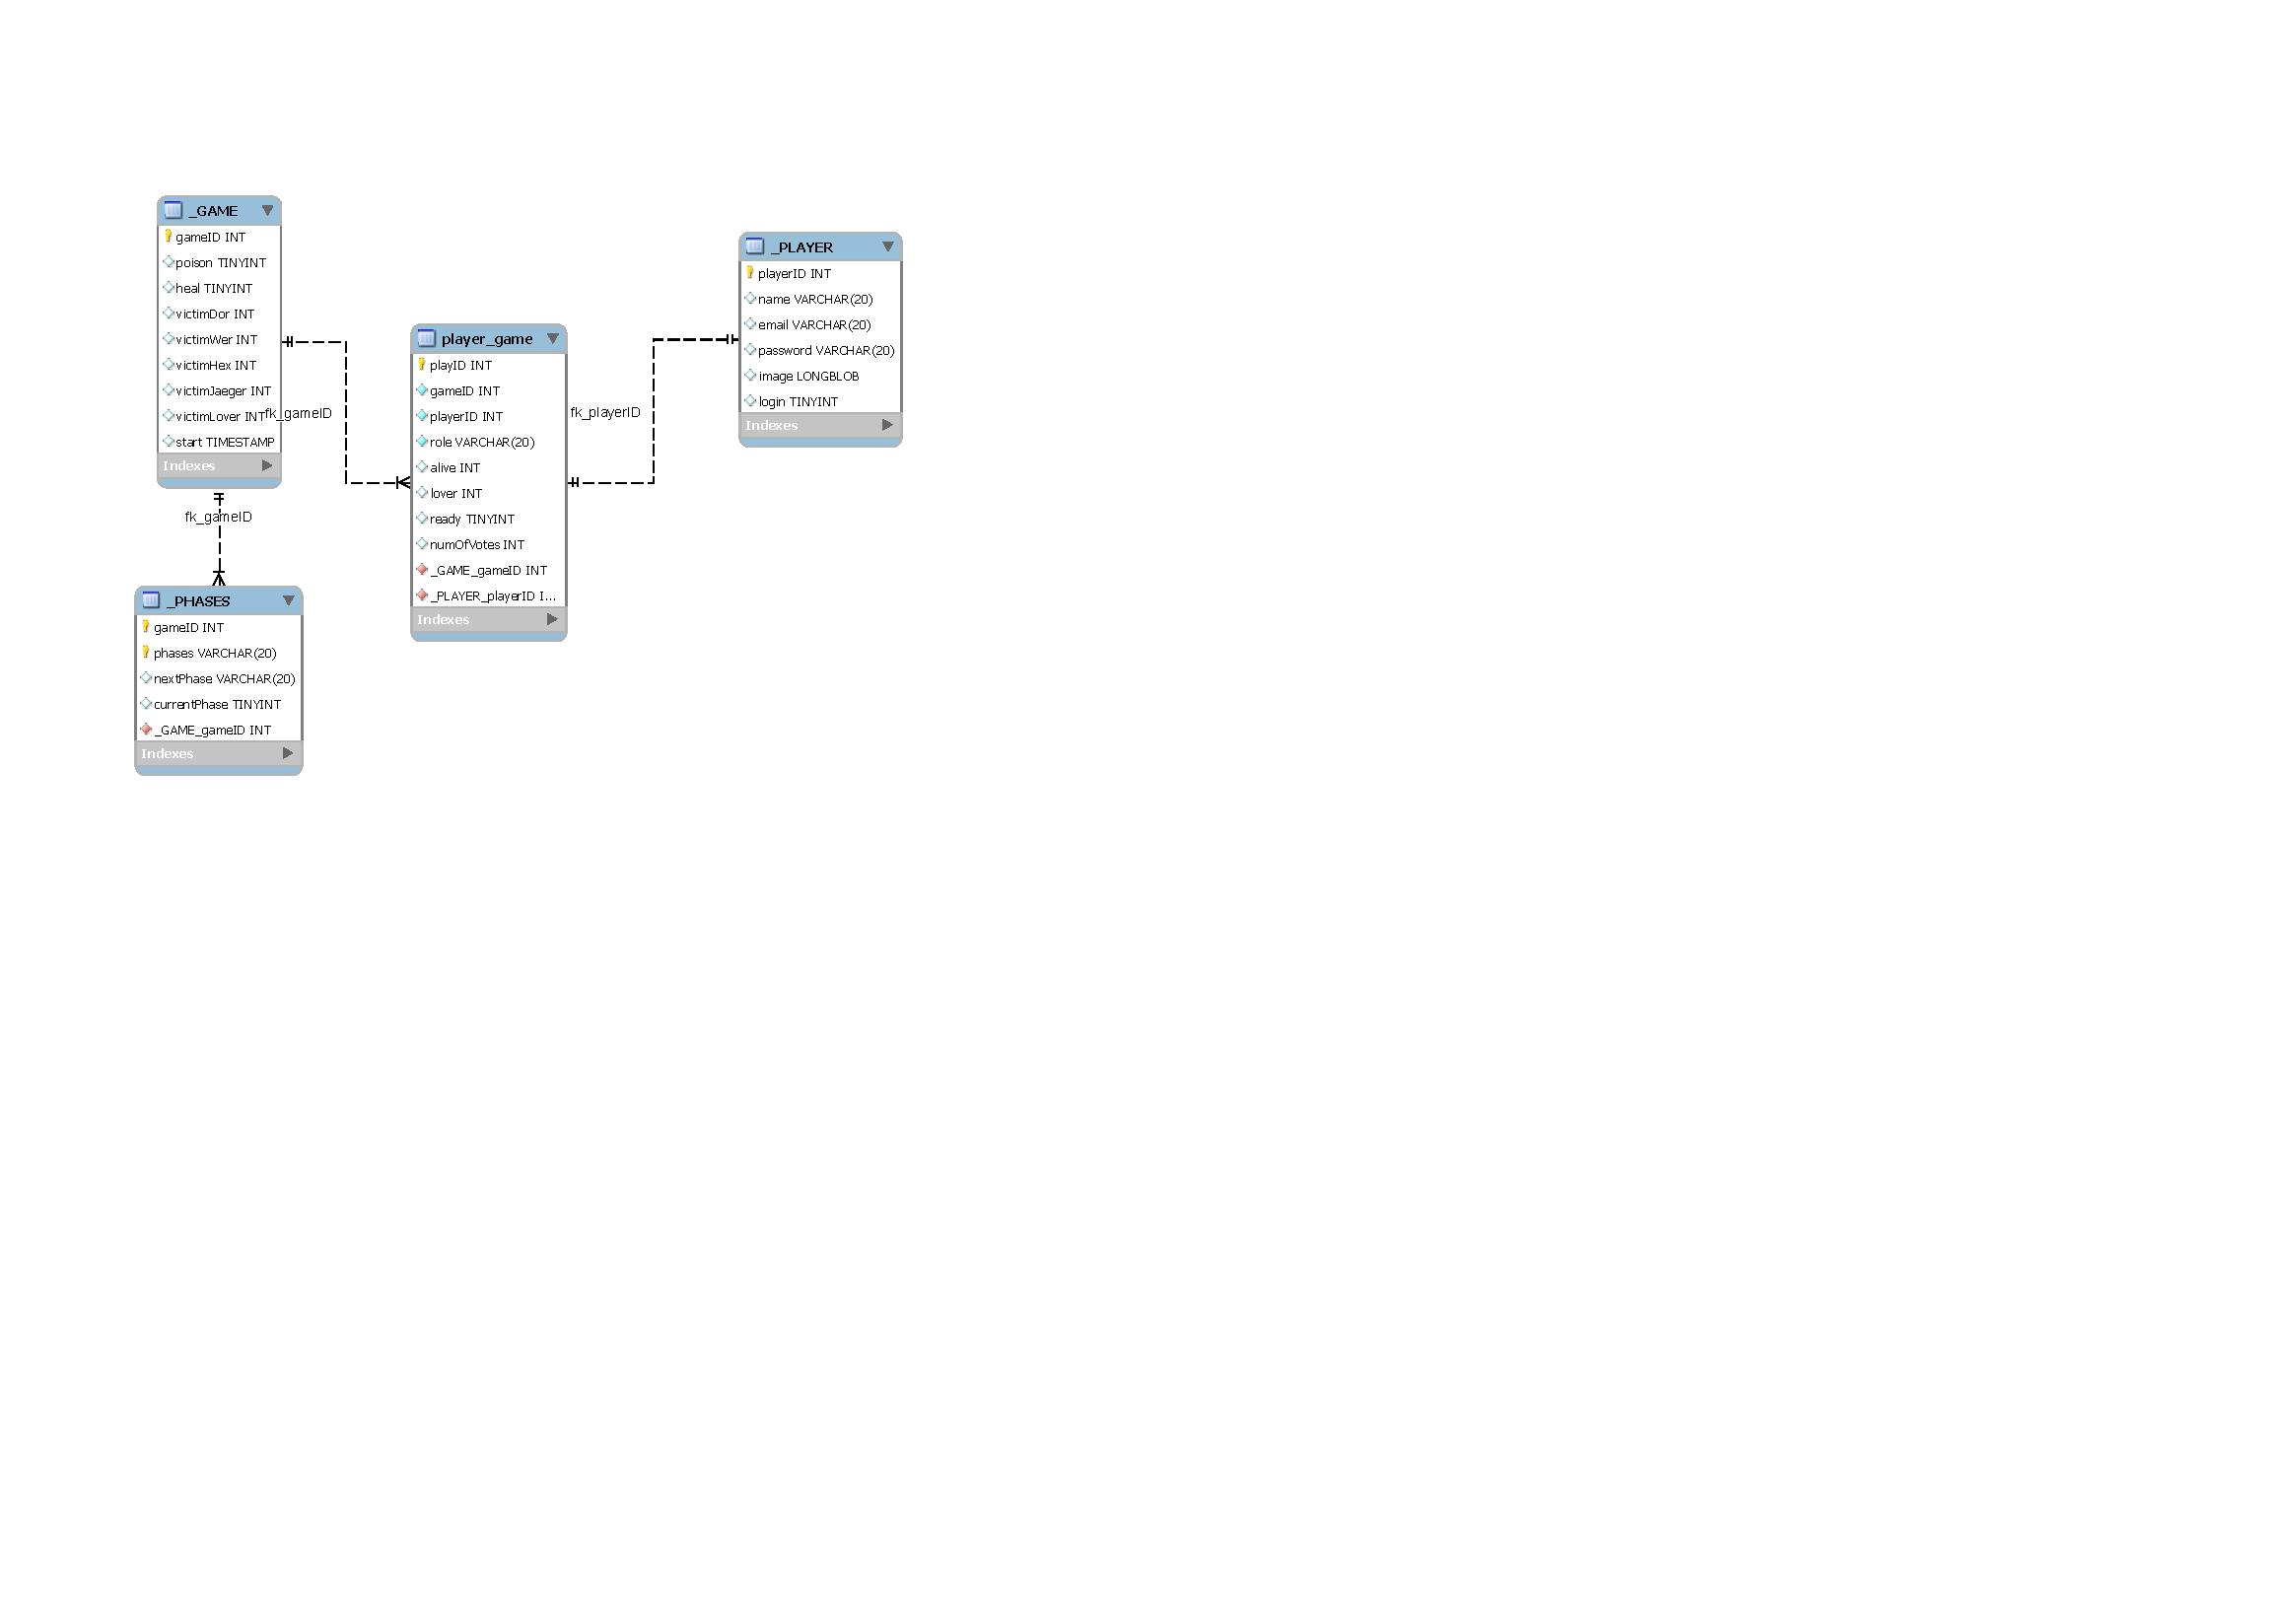
\includegraphics[height = 10 cm, width = 14cm]{DB_Schema}
  \caption{Datenbankschema}
\end{figure}	

\end{document}

